\section{Technical details}

In this chapter, the code architecture and the framework that was created to accelerate this research are described. Then, the chapter describes the hardware used and dives deep into details of benchmarks used to test proposed solutions from the next chapter.

\subsection{HumbleRL framework}

Reinforcement Learning scientists tend to write the entire code from scratch by themselves, instead of using existing RL frameworks. This is justified by the fact, that the commonly available frameworks are not flexible enough for intended experiments or require a specific backend like TensorFlow, which might be disfavored.
HumbleRL \cite{Code.HRL} was created with this problem in mind. Its simple API allows to perform a variety of RL experiments without any restrictions on the algorithms used. Since the backend is not tied to any specific technology, it is possible to mix different neural network frameworks or not use them at all. HumbleRL provides the boilerplate code of RL loop in fig.\ref{Fig.RL} and determines the common interfaces between an agent and an environment, the rest is designed by the user.

Framework architecture is depicted in fig. \ref{Fig.HRL_architecture}. An agent is represented by the Mind class. The Mind encapsulates action planning logic and provides it via the plan method. In order to learn, the agent acts in an environment represented by the Environment class. The Environment provides methods for resetting, taking steps, rendering and getting information about the environment. The MDP class provides the same methods like the environment, and in principle the Environment can be created from the MDP, but additionally it allows direct access to the sample transition model, see the section \ref{Sec.RL}. \\
The framework includes a factory function that creates and returns e.g. wrapped OpenAI Gym environment. The agent is not usually presented with raw environment observations. Instead, it looks at states preprocessed by the Interpreter. Different interpreters can be joined together with the ChainInterpreter class. It acts as a preprocessing pipeline, with each subsequent interpreter using the output of a previous one as an input.

\begin{figure}[H]
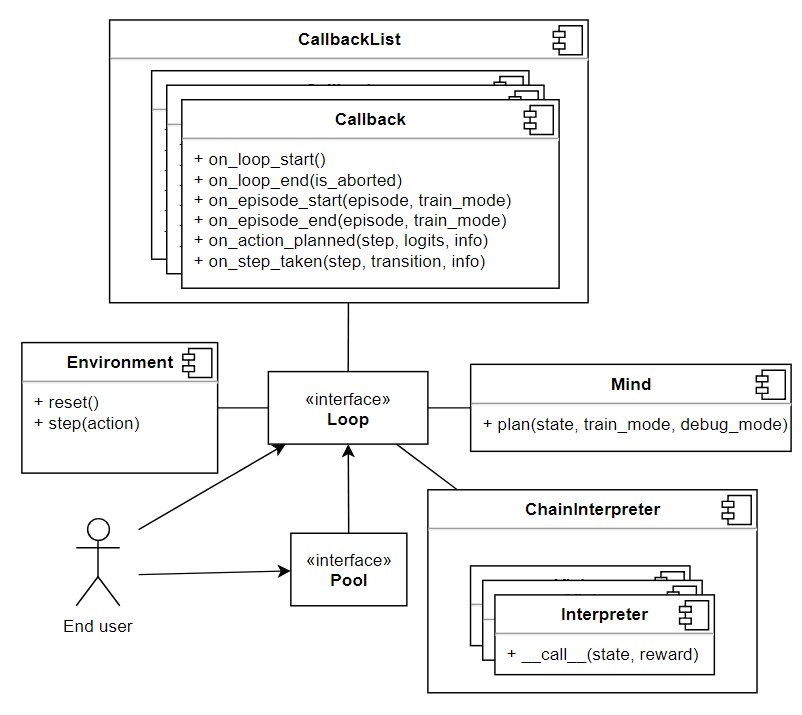
\includegraphics[width=0.6\textwidth,keepaspectratio]{figures/HumbleRL/architecture.png}
\caption{HumbleRL architecture}
\label{Fig.HRL_architecture}
\end{figure}

Framework user does not need to call all of those methods directly, those are utilized by the loop function. This function gets an action from the Mind, executes it in the Environment and then next observation is preprocessed with the Interpreter in preparation for the next step. To extend basic loop functionality, user can define callbacks that implement the Callback interface. Callbacks can react to events:
\begin{itemize}
\item at the beginning and ending of the loop,
\item at the beginning and ending of each episode,
\item after action is planned by the Mind,
\item after step is taken in the Environment.
\end{itemize}
Callbacks are accumulated in the CallbackList. The entire loop function logic is shown in fig. \ref{Fig.HRL_loop}.
Parallel version of loop function is available as the pool function. It uses predefined number of workers to execute a pool of Minds in their own Environments in parallel.

\begin{figure}[H]
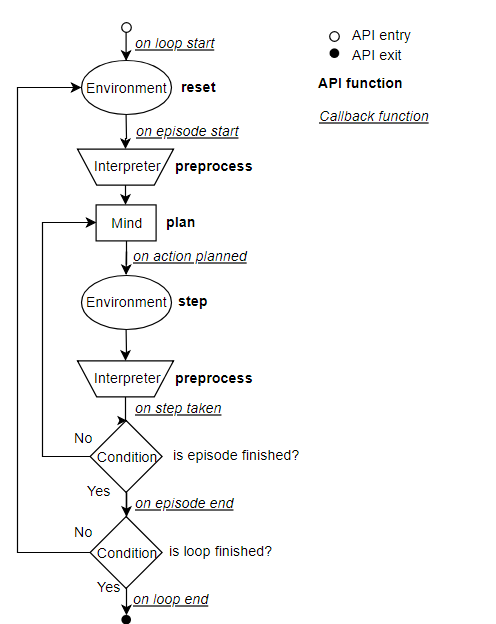
\includegraphics[width=0.6\textwidth,keepaspectratio]{figures/HumbleRL/loop.png}
\caption{HumbleRL loop function overview}
\label{Fig.HRL_loop}
\end{figure}

World Models and AlphaZero implementations use this framework and hence can be joined together into one architecture for experiments.

\subsection{Hardware}

This work used DGX Station from NVIDIA to run experiments. It is the workstation with four NVIDIA Tesla V100 Tensor Core GPUs, integrated with a fully-connected four-way NVLink architecture, delivering 500 teraFLOPS of power, enabling faster experimentation. The system run TensorHive \cite{Code.TensorHive} for managing and monitoring computing resources.

This work did not use distributed training or evaluation. Each experiment was run on one GPU, but multiple experiments were run in parallel on multiple GPUs.

This work has been partially supported by Statutory Funds of Electronics, Telecommunications and Informatics Faculty, Gdansk University of Technology, which provided access to DGX Station deep learning server.

\subsection{Benchmarks}

\subsubsection{Arcade Learning Environment} \label{Sec.ALE}

The Arcade Learning Environment (ALE) has became a platform for evaluating artificial intelligence agents. Originally proposed by Bellemare et. al. \cite{Code.ALE}, the ALE makes available dozens of Atari 2600 games for an agent training and evaluation. The agent is expected to do well in as many games as possible without game-specific information, generally perceiving the environment through a video stream which makes the problem partially observable as already mentioned in the section \ref{Sec.POMDP}. Atari 2600 games are excellent environments for evaluating AI agents for three main reasons: they are varied enough to provide multiple different tasks, requiring general competence, they are interesting and challenging for humans and they are free of experimenter’s bias, having been developed by an independent party.

In the context of the ALE, a discrete action is a number in range from 0 to 17 inclusive which encodes the composition of a joystick direction and an optional button press. The agent observes a reward signal, which is typically the change in the player’s score (the difference in score between the previous time step and the current time step), and an observation $o_t \in O$ of the environment. This observation can take form of a single 210 × 160 image and/or the current 1024-bit RAM state. Because a single image typically does not satisfy the Markov property the ALE is formalised as POMDP. Observations and the environment state are distinguished, with the RAM data being the real state of the emulator. A frame (as a unit of time) corresponds to 1/60th of a second, the time interval between two consecutive images rendered to the television screen. The ALE is deterministic, which means that given a particular emulator state $s$ and a action $a$ there is a unique next state $s'$, that is, $P^a_{ss'} = p(s' | s, a) = 1$.

Agents interact with the ALE in an episodic fashion. An episode begins by resetting the environment to its initial configuration, $s_0$, and ends at a given endpoint depending on a game. The primary measure of an agent’s performance is the score achieved during an episode, namely the undiscounted sum of rewards for that episode. While this performance measure is quite natural, it is important to realize that score is not necessarily an indicator of AI progress. In some games, agents can exploit the game's mechanics to maximize sum of rewards, but not complete the game's goal in human's understanding \cite{Study.FaultyReward}.

Common preprocessing techniques include frame skipping \cite{Study.FrameSkipping} which restricts the agent decision points by repeating a selected action for 4 consecutive frames. It is used in reinforcement learning \cite{Algo.DQN} to reduce the planning horizon and provide a clearer learning signal to the model, but it also speeds up execution.

This work uses ALE through OpenAI Gym API \cite{Code.OpenAIGym}, specifically two Atari games are used as benchmarks: Boxing and Freeway.

Boxing is a video game based on the sport of boxing. Boxing shows a top-down view of two boxers, one white and one black. When close enough, a boxer can hit his opponent with a punch. This causes his opponent to reel back slightly and the boxer scores a point, a reward of 1. In the other situation, when the boxer gets hit, he gets a negative reward of -1. There are no knockdowns or rounds. A match is completed either when one player lands 100 punches (a 'knockout') or two minutes have elapsed. In the case of a decision, the player with the most landed punches is the winner. Ties are possible. 
While the gameplay is simple, there are subtleties, such as getting an opponent on the 'ropes' and 'juggling' him back and forth between alternate punches. 

\begin{figure}[H]
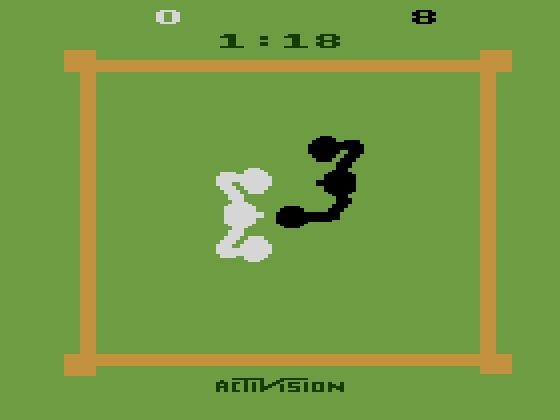
\includegraphics[width=0.5\textwidth,keepaspectratio]{figures/Boxing.jpg}
\caption[Boxing]{Example of Boxing level}
\label{Fig.Boxing}
\end{figure}

In Freeway an agent controls a chicken who can be made to run across a ten lane highway filled with traffic in an effort to "get to the other side." Every time a chicken gets across a reward of 1 is earned by the agent. If hit by a car, then a chicken is forced back slightly. The goal is to score as much points as possible in the two minutes. The chicken is only allowed to move up or down. 
The major challenge in this environment are sparse rewards. The agent scores only when successfully crosses the highway, which is not a trivial task.

\begin{figure}[H]
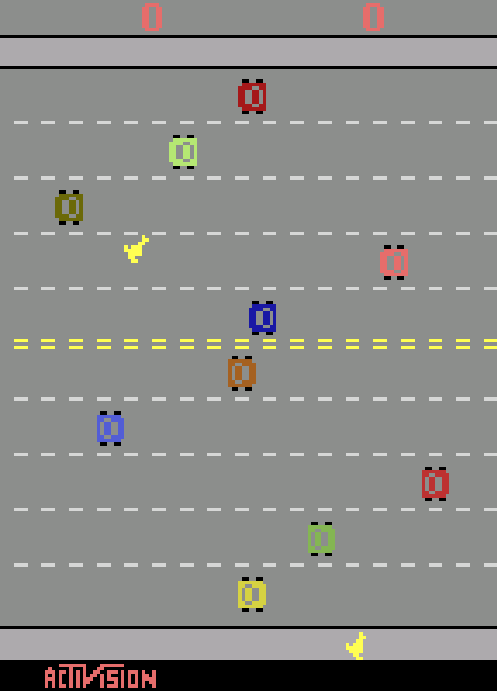
\includegraphics[width=0.5\textwidth,keepaspectratio]{figures/Freeway.png}
\caption[Freeway]{Example of Freeway level}
\label{Fig.Freeway}
\end{figure}

\subsubsection{Sokoban}

Sokoban is a classic planning problem which is not strictly part of ALE, but it can be added to OpenAI Gym API \cite{Code.Sokoban}. It is a challenging one-player puzzle game in which the goal is to navigate a grid world maze and push boxes onto target tiles. A Sokoban puzzle is considered solved when all boxes are positioned on top of target locations. The player can move in all 4 cardinal directions and only push boxes into an empty space (as opposed to pulling). For this reason many moves are irreversible and mistakes can render the puzzle unsolvable. A human player is thus forced to plan moves ahead of time. Artificial agents should similarly benefit from a learned model and simulation.

Despite its simple rule set and fully observability - each game frame shows all blocks, targets, walls and agent positions and states - Sokoban is an incredibly complex game for which no general solver exists. It can be shown that Sokoban is NP-Hard and PSPACE-complete \cite{Benchmark.Sokoban}. Sokoban has an enormous state space that makes it inassailable to exhaustive search methods. An efficient automated solver for Sokoban must have strong heuristics, just as humans utilize their strong intuition, so that it is not overwhelmed by the number of possible game states.

The implementation of Sokoban used for those experiments procedurally generates a new level each episode. This means an agent cannot memorize specific puzzles. Together with the planning aspect, this makes for a very challenging environment. While the underlying game logic operates in a 10 × 10 grid world, with 7 possible elements in each grid ~\ref{Fig.Sokoban_elements}, agents were trained directly on RGB sprite graphics. Fig.~\ref{Fig.Sokoban} shows an example of Sokoban level with 4 boxes. \\
Finishing the game by pushing all blocks on the targets gives a reward of 10 in the last step. Also pushing a box on or off a target gives a reward of 1 or -1 respectively. In addition, a reward of -0.1 is given for every step which penalizes solutions with many steps.

\begin{figure}[H]
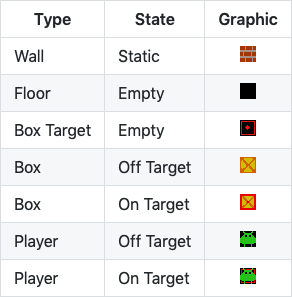
\includegraphics[width=0.4\textwidth,keepaspectratio]{figures/Sokoban_elements.png}
\caption[Sokoban elements]{Table with Sokoban possible elements in each grid, further referred to as blocks.}
\label{Fig.Sokoban_elements}
\end{figure}

\begin{figure}[H]
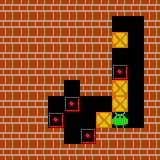
\includegraphics[]{figures/Sokoban.png}
\caption[Sokoban]{Example of Sokoban level}
\label{Fig.Sokoban}
\end{figure}
